\begin{frame}
	\frametitle{Interaktion Hydrosphäre, Kryosphäre und Atmosphäre}
	\begin{columns}
		\column{.6\linewidth}
		\begin{figure}
			\centering
			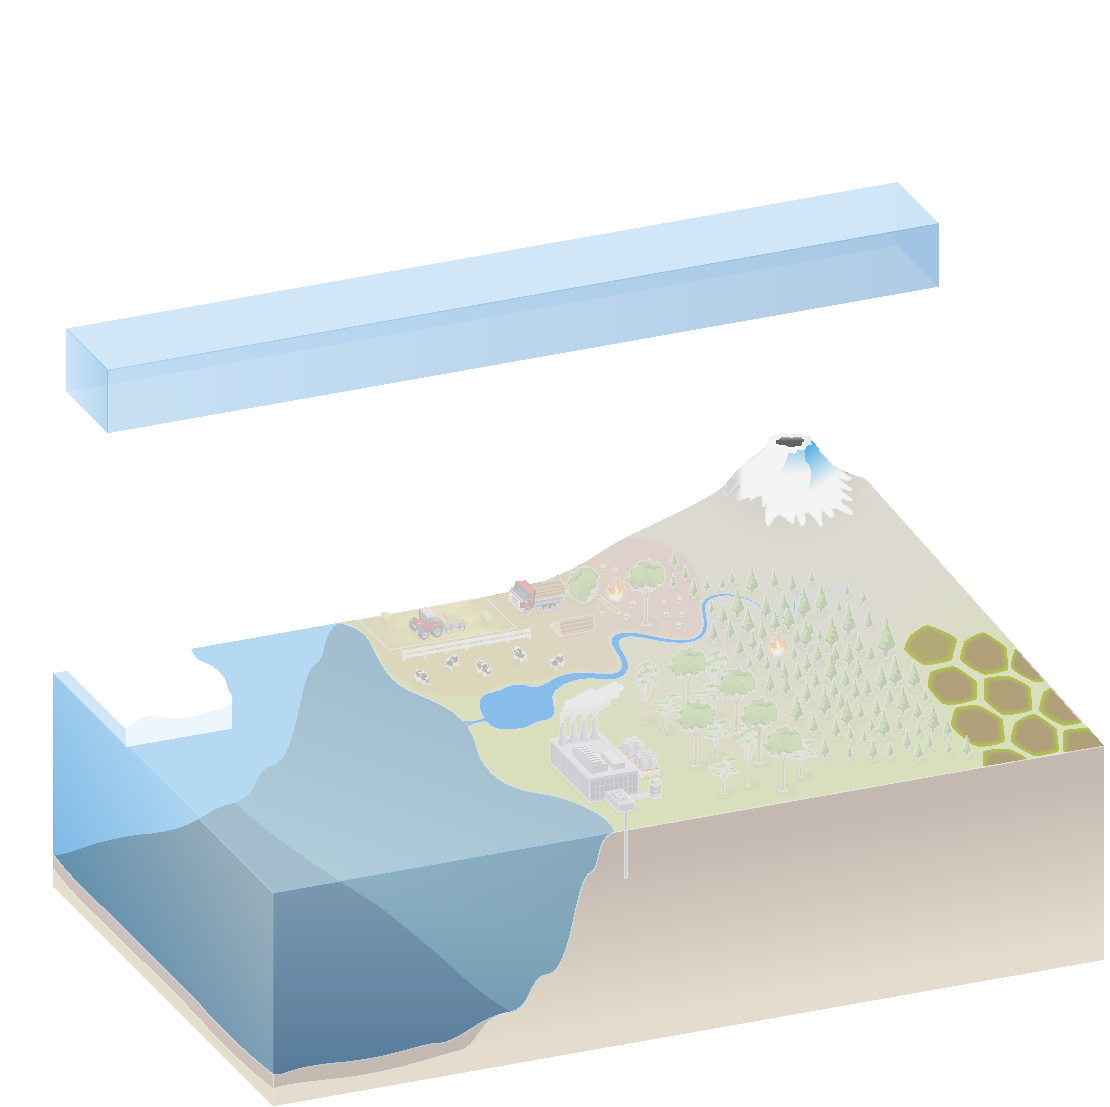
\includegraphics[trim={1cm 0cm 0cm 3cm}, clip, width=0.7\linewidth]{%
	        bilder/climate_components/global_climate_components_interaction_atmo_hydro_kryo.pdf}
			\caption{Interaktion Hydrosphäre, Kryosphäre und Atmosphäre}
		\end{figure}
		\column{.4\linewidth}
		\begin{itemize}
			\item Verringerter Albedo-Effekt
			\item Abgeschwächte Konvektion
			\item Abgeschwächte Ozeanströmung und Winde
			\item Anstieg des Meeresspiegels
			\item Massive Freisetzung von Treibhausgasen aus den Senken Ozean und Permafrost
			\item Trägheit führt zu verzögertem Eintreten der Änderungen
		\end{itemize}
	\end{columns}
	\begin{block}{}
			$\rightarrow$ Insgesamt: eine Verstärkung des Treibhauseffekt mit weiteren noch unabsehbaren Folgen
	\end{block}

	\note{
		\begin{itemize}
			\item[] links an den Pfeilen sind die Wechselwirkungen notiert - z.B. Eis-Ozean-Verbindung (Konvektion)
			\item[] rechts sieht man die allgemeinen Elemente der Komponenten Hydrosphäre und Kryosphäre
			\item[] diese Elemente hängen offensichtlich zusammen und bedingen sich gegenseitig
			\item[] Das Schmelzen der Polkappen und Auftauen des Permafrostes ist ein deutliches Signal
			\item[] Wie gesagt, kann ein einmal in Gang gesetztes Abtauen schwer aufzuhalten sein
			\item[] Die Effekte können deutlich später auftreten
		\end{itemize}
	}
\end{frame}
